% Appendix frames support questions after the closing slide.
\section*{Appendix}




% Source. Background 2.1, eq:categorical-likelihood and eq:likelihood-factorization.
% Speaking notes
% The categorical distribution assigns each label the corresponding class probability from the network output.
% In this product over classes, the indicator selects the probability of the observed label.
% That class has exponent one. Every other class has exponent zero and contributes a factor of one.
% We then multiply the observed-label probabilities across conditionally independent training examples to obtain the likelihood.
\begin{frame}{Categorical Observation Model}
    \label{frm:backup-categorical-observation}
    \begin{itemize}
    \item For input $x$ and weights $w$, $f(x;w)$ lists probabilities for $C$ classes.
    \item $y$ is the label. $\mathbb I[y=c]$ is 1 when $y=c$ and 0 otherwise.
    \end{itemize}
    % Copied from thesis eq:categorical-likelihood.
    \[
    p(y\mid x,w)=\mathrm{Cat}\bigl(y\mid f(x;w)\bigr)
    =\prod_{c=1}^{C}f_c(x;w)^{\mathbb I[y=c]}=f_y(x;w).
    \]
    \begin{itemize}
    \item $D$ contains $N$ labelled pairs $(x_i,y_i)$.
    \item Conditional independence gives the product over observations.
    \end{itemize}
    % Thesis eq:likelihood-factorization and eq:categorical-likelihood.
    \[
    p(D\mid w)=\prod_{i=1}^{N}p(y_i\mid x_i,w)=\prod_{i=1}^{N}f_{y_i}(x_i;w).
    \]
    \end{frame}
    
    
    % Source. Author-requested supporting theory for Methods 4.2.1, sec:edl-model-setup.
    % Sensoy et al. 2018, Section 3, pp. 3--4. Jøsang 2016 UAI tutorial, slides 12, 20, 29 and 33--35.
    % Verified primary-source details are in VERIFIED_SOURCES.md.
    % Speaking notes
    % Consider a prediction of fifty percent bird and fifty percent frog.
    % The model might have little evidence for either class.
    % Alternatively, it might have substantial but balanced evidence for both classes.
    % The class probabilities alone do not distinguish these situations.
    % Subjective logic lets us represent this distinction through assigned and unassigned belief.
    % With little evidence, most belief remains unassigned. With strong evidence, more belief is assigned to the supported classes.
    % Base probabilities specify how unassigned belief contributes to the predicted class probabilities.
    % The two situations can therefore give the same prediction, despite different amounts of unassigned belief.
    % This describes what the representation can express. It does not guarantee that a trained network estimates evidence correctly.
    % The following example makes the distinction explicit using the same notation.
    \begin{frame}{Theory of Evidence and Subjective Logic}
    \label{frm:backup-subjective-logic}
    \begin{itemize}
    \setlength{\itemsep}{1mm}
    \item A $(0.5,0.5)$ bird--frog class probability prediction can reflect
    \begin{itemize}
    \item \textbf{Little evidence} for either class.
    \item \textbf{Evidence} that supports both classes equally.
    \end{itemize}
    \item For $C$ classes, subjective logic represents the model's belief about the class label using
    \begin{itemize}
    \item $b_c$, belief assigned to class $c$.
    \item $u$, belief not assigned to any individual class.
    % Sensoy Section 3. Jøsang slide 20. Class count is C in thesis notation.
    \[
    b_c\geq0,\qquad u\geq0,\qquad \sum_{c=1}^{C}b_c+u=1.
    \]
    \item $a_c$, base probability is fraction of unassigned belief allocated to class $c$
    \[
    a_c\geq0,\qquad \sum_{c=1}^{C}a_c=1.
    \]
    \end{itemize}
    \item Probability of class $c$ is a function of its \textbf{assigned} and \textbf{unassigned} belief,
    \[
    p(y=c)=\underbrace{b_c}_{\text{assigned belief}}
    +\underbrace{a_cu.}_{\text{share of unassigned belief}}
    \]
    \end{itemize}
    \end{frame}
    
    % Source. Author-requested illustration of Jøsang 2016, slides 12 and 20.
    % Values follow from the projected probability p(y=c)=b_c+a_c u.
    % Supporting context. Methods 4.2.1, sec:edl-model-setup. This is not an experimental result.
    % Speaking notes
    % Suppose the two possible classes are bird and frog.
    % First, we have no evidence that supports either class specifically.
    % Class belief means the mass assigned to one particular class. Here both class belief masses are zero.
    % Unassigned belief is the mass left without choosing an individual class. Here all the mass remains unassigned.
    % We still need class probabilities. Base probabilities specify how to distribute the unassigned mass.
    % We choose equal base probabilities, so half goes to bird and half to frog.
    % Each class therefore gets zero assigned belief plus half the unassigned mass, giving fifty percent.
    % Now consider a different opinion. Half the belief is assigned to bird and half to frog.
    % Nothing remains unassigned. Each class still receives fifty percent probability.
    % The prediction is identical, but one opinion leaves all belief unassigned and the other assigns it all.
    % Thus, no unassigned belief does not mean we know which class label applies.
    % In EDL, fully assigned balanced belief is approached as equal evidence increases without bound.
    % Finite EDL evidence always leaves some unassigned belief.
    \begin{frame}{Theory of Evidence and Subjective Logic Example}
    \label{frm:backup-belief-example}
    \setlength{\abovedisplayskip}{4pt}
    \setlength{\belowdisplayskip}{4pt}
    \begin{itemize}
    \setlength{\itemsep}{3mm}
    \item Consider $C=2$ classes, bird ($c=1$) and frog ($c=2$).
    \begin{itemize}
    \item \textbf{Base probabilities $a_c$} distribute unassigned belief. Choose $a_1=a_2=0.5$.
    \end{itemize}
    \item \textbf{No assigned belief}
    \begin{itemize}
    \item \textbf{Class belief $b_c$} assigned to class $c$.
    No belief assigned $b_1=b_2=0$.
    \item \textbf{Unassigned belief} $u=1$ (since $\sum_c b_c+u=1$).
    \[
    p(y=c)=b_c+a_cu=0+0.5\times1=0.5,
    \qquad c\in\{1,2\}.
    \]
    \item $(0.5,0.5)$ predicted class probability reflects \textbf{no evidence supporting belief for either class}.
    \end{itemize}
    \item \textbf{Belief assigned}
    \begin{itemize}
    \item Suppose \textbf{evidence supports assigning belief} to each class. $b_1=b_2=0.5$ and $u=0$.
    \[
    p(y=c)=b_c+a_cu=0.5+0.5\times0=0.5,
    \qquad c\in\{1,2\}.
    \]
    \item $(0.5,0.5)$ predicted class probability reflects \textbf{evidence supporting belief for equal classes.}
    \end{itemize}
    \end{itemize}
    \end{frame}
    
    % Source. Sensoy et al. 2018, Section 3, pp. 3--4, and Section 4, opening paragraphs.
    % Background 2.2, eq:dirichlet-density. Methods 4.2.1, eq:edl-softplus-evidence,
    % eq:edl-dirichlet-concentration and eq:edl-dirichlet.
    % Speaking notes
    % We have described subjective belief. We now construct the distribution that EDL uses to represent it.
    % The network predicts a nonnegative amount of support for each class, called evidence.
    % These outputs are learned from labelled examples. They are not observed counts or class probabilities.
    % We first need a baseline for the case where there is no evidence for any class.
    % EDL chooses a uniform Dirichlet distribution over possible class-probability vectors.
    % This distribution has all concentration parameters equal to one.
    % Its density is constant because each exponent is the concentration parameter minus one.
    % EDL adds the learned evidence to these baseline parameters, giving one plus evidence.
    % The resulting concentration vector specifies the Dirichlet distribution for the input.
    % This distribution describes possible class probabilities, not possible evidence outputs.
    % The baseline is a modelling choice, not a requirement of subjective logic alone.
    % In our softplus implementation, zero evidence is approached only as a limit.
    % Next, we read assigned belief, unassigned belief and base probabilities from the Dirichlet parameters.
    \begin{frame}{Evidential Deep Learning }
    \label{frm:backup-edl-evidence-meaning}
    \begin{itemize}
    \setlength{\itemsep}{5mm}
    \item The network outputs evidence $e_c(x;w)\geq0$, \textbf{learned support for class $c$}.
    \item EDL chooses a \textbf{uniform Dirichlet distribution at zero evidence}.
    \begin{itemize}
    \item Baseline concentration of one for every class.
    \end{itemize}
    \item Learned evidence adds to this baseline,
    % Thesis eq:edl-dirichlet-concentration. Sensoy Section 3.
    \[
    \alpha_c(x;w)=\underbrace{1}_{\text{baseline}}
    +\underbrace{e_c(x;w).}_{\text{learned class evidence}}
    \]
    \item Concentration parameters specify a distribution over random class probability vectors $\pi$,
    % Thesis eq:edl-dirichlet.
    \[
    p(\pi\mid x,w)=\mathrm{Dir}\bigl(\pi\mid\alpha(x;w)\bigr).
    \]
    \end{itemize}
    \end{frame}
    

% Source. Background 2.2, eq:dirichlet-density and eq:general-dirichlet-mean.
% Sensoy et al. 2018, Section 3, pp. 3--4, uniform baseline at zero evidence.
% Figure. scripts/build_edl_baseline.py. Samples from the Dirichlet density, not experimental results.
% Speaking notes
% Each green dot represents three class probabilities. The corners give one class probability one.
% The red dot marks the mean, one third for each class, in all three triangles.
% 1) Small positive concentration parameters favour the corners. One class receives almost all the probability, but each corner is equally favoured.
% 2) Parameters of one give constant density across the triangle. Equal areas have equal probability.
% This favours neither balanced nor unequal class probabilities.
% 3) Parameters of five favour vectors near the centre, with roughly 1/3 probability for each class.
% None favours a particular class. They differ in which probability vectors they favour.
% Zero concentration parameters are invalid. The left plot uses small positive values.
% EDL chooses the uniform density as its zero evidence baseline. Adding one implements this choice.
\begin{frame}{The Dirichlet Baseline at Zero Evidence}
\label{frm:appendix-edl-zero-evidence}
\begin{itemize}
    \setlength{\itemsep}{2mm}
\item Each dot is a sampled class-probability vector.
\begin{itemize}
\item Vertices assign probability one to a class. 
\item The centre assigns $1/3$ probability to each class.
\end{itemize}
\begin{center}
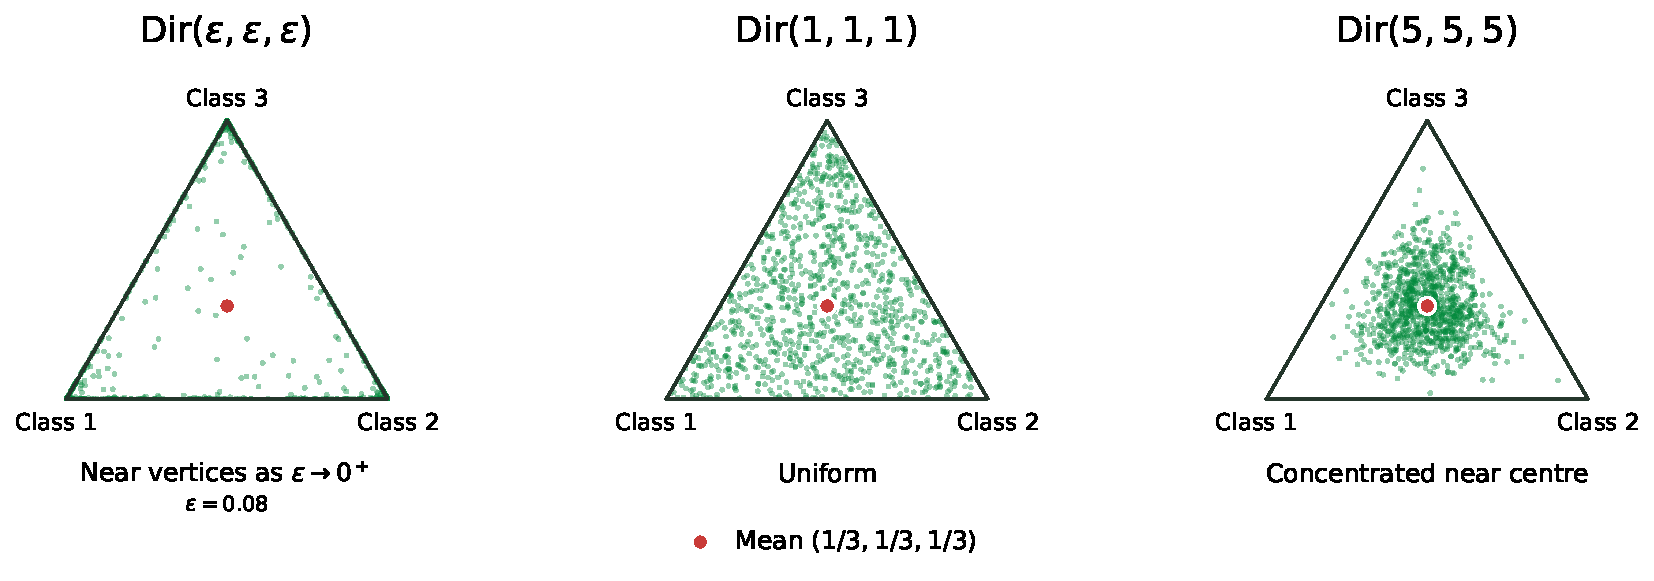
\includegraphics[width=.85\textwidth]{figures/edl_zero_evidence_baselines.pdf}
\end{center}
\item EDL chooses \textbf{uniform density at zero evidence}
\end{itemize}
\end{frame}

    % Source. Sensoy et al. 2018, Section 3, Eqs. (1)--(2) and inverse belief mapping after Eq. (1).
    % Jøsang 2016 UAI tutorial, slides 20--24, opinion and Dirichlet correspondence.
    % Methods 4.2.1, eq:edl-dirichlet-concentration and eq:edl-predictive.
    % Speaking notes
    % We adopt the interpretation specified by Sensoy and colleagues.
    % Learned evidence supplies support assigned to individual classes. The unit baseline represents unassigned belief.
    % The network learns evidence values. The meaning of the belief quantities is part of the chosen model.
    % We divide the evidence for each class by total concentration to obtain its assigned belief.
    % Unassigned belief is what remains after summing all assigned belief.
    % The remaining baseline has one unit per class, giving the number of classes divided by total concentration.
    % Each class receives an equal share of that baseline, so its base probability is one divided by the number of classes.
    % These are the assigned belief, unassigned belief and base probabilities from our earlier example.
    % We now calculate a class probability by adding its assigned belief and its share of unassigned belief.
    % The result equals the Dirichlet mean. The equation shows the same class probability in both representations.
    % The opinion also retains unassigned belief, which the class probabilities alone do not specify.
    % This mapping uses EDL's chosen baseline. Unassigned belief is not the thesis distributional mutual information.
    \begin{frame}{Subjective Logic Interpretation of Dirichlet Model}
    \label{frm:backup-opinion-dirichlet}
    \label{frm:backup-edl-evidence}
    \setlength{\abovedisplayskip}{5pt}
    \setlength{\belowdisplayskip}{5pt}
    \begin{itemize}
    \setlength{\itemsep}{2mm}
    \item Following Sensoy et al. (2018) normalised evidence gives \textbf{assigned class belief}, normalised baseline gives \textbf{unassigned belief}.
    \begin{itemize}
    \item Normalise by $\alpha_0(x;w)=\sum_c\alpha_c(x;w)$ gives belief masses,
    % Sensoy Eq. (1). The second line follows from sum_c b_c+u=1.
    \[
    \begin{aligned}
    b_c(x;w)&=\frac{e_c(x;w)}{\alpha_0(x;w)},\\[2mm]
    u(x;w)&=1-\sum_{c=1}^{C}b_c(x;w)=\frac{C}{\alpha_0(x;w)}.
    \end{aligned}
    \]
    \item $a_c=1/C$ base probabilities $\forall c$ since each class has one baseline unit.
    \end{itemize}
    % \item Both representations give the same class probabilities.
    % % Jøsang slide 20. Sensoy Eq. (2). Thesis eq:edl-predictive, evaluated at class c.
    % \[
    % \underbrace{p(y=c\mid x,w)}_{\text{class probability}}
    % =\underbrace{b_c(x;w)+a_cu(x;w)}_{\text{subjective logic}}
    % =\underbrace{\frac{\alpha_c(x;w)}{\alpha_0(x;w)}}_{\text{Dirichlet mean}}.
    % \]
    \item Gives \textbf{subjective logic interpretation} of Dirichlet--categorical observation model,
    \[
    \underbrace{p(y=c\mid x,w)}_{\text{observation model}}
    =
    \underbrace{b_c(x;w)+a_cu(x;w)}_{\text{subjective logic}}
    =
    \underbrace{\frac{\alpha_c(x;w)}{\alpha_0(x;w)}.}_{\text{Dirichlet mean}}
    \]
    \end{itemize}
    \end{frame}

    
% Source. Background 2.6, eq:shannon-entropy, eq:expected-conditional-entropy,
% eq:mutual-information and eq:general-entropy-decomposition.
% Speaking notes
% Entropy measures uncertainty about the class label.
% Suppose another quantity becomes known. We calculate the remaining label entropy for each possible value of that quantity.
% Averaging gives expected conditional entropy.
% The difference from the original entropy is mutual information, the average reduction obtained by knowing that quantity.
% Rearranging gives the entropy decomposition shown below.
\begin{frame}{Entropy and its Decomposition}
\label{frm:backup-entropy-decomposition}
\setlength{\abovedisplayskip}{4pt}
\setlength{\belowdisplayskip}{4pt}
\begin{itemize}
\setlength{\itemsep}{5mm}
\item \textbf{Entropy} measures label uncertainty,
% Thesis eq:shannon-entropy.
\[
\mathcal H[p(y)]=-\sum_{c=1}^{C}p(y=c)\log p(y=c).
\]
\item \textbf{Expected conditional entropy} averages what remains when the random variable $\xi$ is known,
% Thesis eq:expected-conditional-entropy.
\[
\mathcal H[y\mid\xi]=\mathbb E_{p(\xi)}\!\left[\mathcal H[p(y\mid\xi)]\right].
\]
\item \textbf{Mutual information} is the average reduction from knowing $\xi$,
% Thesis eq:mutual-information.
\[
\mathcal I(y;\xi)=\mathcal H[p(y)]-\mathcal H[y\mid\xi],
\]
\end{itemize}
% Thesis eq:general-entropy-decomposition.
\[
\underbrace{\mathcal H[p(y)]}_{\text{total}}
=\underbrace{\mathcal H[y\mid\xi]}_{\text{average remaining}}
+\underbrace{\mathcal I(y;\xi).}_{\text{average reduction}}
\]
\end{frame}

% Source. Background 2.7, eq:weight-level-decomposition,
% eq:fixed-weight-decomposition and eq:three-way-decomposition.
% Speaking notes
% We apply the generic decomposition first to the weights, then to class probabilities at given weights.
% The aleatoric term averages the label entropy remaining with known class probabilities.
% The distributional term averages the reduction obtained by knowing those probabilities at given weights.
% The epistemic term measures the average reduction obtained by knowing the weights.
% The input and training data remain fixed throughout.
\begin{frame}{Decomposition of Predictive Uncertainty}
\label{frm:backup-three-way-decomposition}
\begin{itemize}
\setlength{\itemsep}{4mm}
\item Apply the decomposition to weights $w$, then to class probabilities $\pi$ given $w$.
\item Given input $x$ and training data $D$,
\end{itemize}
% Thesis eq:three-way-decomposition. Only line breaks are changed.
\begin{align*}
\underbrace{\mathcal H[p(y\mid x,D)]}_{\text{predictive}}
&=\underbrace{\mathbb E_{p(w\mid D)}\!\left[
\mathbb E_{p(\pi\mid x,w)}\!\left[\mathcal H[\mathrm{Cat}(y\mid\pi)]\right]\right]}_{\text{aleatoric}}\\[4mm]
&\quad+\underbrace{\mathbb E_{p(w\mid D)}\!\left[\mathcal I(y;\pi\mid w)\right]}_{\text{distributional}}\\[4mm]
&\quad+\underbrace{\mathcal I(y;w)}_{\text{epistemic}}.
\end{align*}
\end{frame}

% Source. Background 2.8 and 2.9, eq:aleatoric-epistemic-decomposition,
% eq:aleatoric-distributional-split and sec:bg-dirichlet-point-estimate.
% Speaking notes
% For the categorical Bayesian network, a given input and set of weights specify one class-probability vector.
% Knowing the vector then adds no information, so the distributional term is zero.
% The deterministic Dirichlet network instead uses one fitted weight vector.
% Knowing those weights adds no information, so the epistemic term is zero.
% These zeros follow from model structure. They do not show that the corresponding source is absent from the problem.
\begin{frame}{Model-Specific Uncertainty Decompositions}
\label{frm:backup-model-decompositions}
\begin{itemize}
\item \textbf{Categorical BNN}\quad Given $x,w$, $p(\pi=f(x;w)|x,w) = 1$.\\
Distributional term is zero.
\end{itemize}
% Thesis eq:aleatoric-epistemic-decomposition.
{\small
\[
\underbrace{\mathcal H[p(y\mid x,D)]}_{\text{predictive}}
=\underbrace{\mathbb E_{p(w\mid D)}\!\left[\mathcal H[\mathrm{Cat}(y\mid f(x;w))]\right]}_{\text{aleatoric}}
+\underbrace{\mathcal I(y;w)}_{\text{epistemic}}.
\]
% where p(y|x,D) is the model's predicted class probabilities for input x and training data D. which is Cat(y|f(x;w))
}
\medskip
\begin{itemize}
\item \textbf{Deterministic Dirichlet network}\quad The weights are fixed at $\hat{w}$.\\
Epistemic term is zero.
\end{itemize}
% Thesis eq:aleatoric-distributional-split.
{\small
\[
\underbrace{\mathcal H[p(y\mid x,\hat{w})]}_{\text{predictive}}
=\underbrace{\mathbb E_{\mathrm{Dir}(\pi\mid\alpha(x;\hat{w}))}\!\left[\mathcal H[\mathrm{Cat}(y\mid\pi)]\right]}_{\text{aleatoric}}
+\underbrace{\mathcal I(y;\pi\mid\hat{w})}_{\text{distributional}}.
\]
% Here p(y|x,\hat{w}) = Cat(y|m(x;\hat{w})) is the predicted label distribution at the fitted weights.
}
\medskip
\begin{itemize}
\item Combining a \textbf{weight posterior} with a \textbf{Dirichlet distribution} for class probabilities allows all three terms.
\end{itemize}
\end{frame}

% Source. Background eq:general-entropy-decomposition, eq:expected-conditional-entropy,
% eq:aleatoric-distributional-split, eq:mean-total-concentration-parameterisation,
% eq:aleatoric-as-function-of-total-concentration and eq:digamma-function.
% Appendix A.1 uses the same generic Dirichlet categorical setup.
% Speaking notes
% Start with the generic identity. Label entropy is the expected entropy remaining after another quantity is known, plus the information it provides.
% For the Dirichlet categorical model, that quantity is the class-probability vector.
% Marginalising this vector gives a categorical label distribution parameterised by the Dirichlet mean.
% Substituting the two distributions gives the predictive entropy split into aleatoric and distributional uncertainty.
% We then name the aleatoric term as a function of total concentration, indexed by the mean vector.
% Its closed form uses the digamma function.
% The decomposition itself does not require a comparison at fixed mean.
% For the propositions that follow, we hold the mean fixed and study how this function changes with total concentration.
\begin{frame}{Backup. Dirichlet Categorical Uncertainty Decomposition}
\label{frm:backup-dirichlet-categorical-split}
\setlength{\abovedisplayskip}{4pt}
\setlength{\belowdisplayskip}{4pt}
\begin{itemize}
\setlength{\itemsep}{4mm}
% \item Generic entropy decomposition
% % Thesis eq:general-entropy-decomposition.
% \[
% \mathcal H[p(y)]=\mathcal H[y\mid\xi]+\mathcal I(y;\xi).
% \]
\item $p(\pi\mid\alpha)=\mathrm{Dir}(\pi\mid\alpha)$, $p(y\mid\pi)=\mathrm{Cat}(y\mid\pi)$, $\alpha_c>0$.
\item Marginalising $\pi$ gives $p(y\mid\alpha)=m_y=\mathrm{Cat}(y\mid m)$ 
\begin{itemize}
\item $m=\alpha/\alpha_0$, $\alpha_0=\sum_c\alpha_c$ 
\end{itemize}
\item Predictive uncertainty decomposes as
\end{itemize}
% Thesis eq:aleatoric-distributional-split, generic form in Appendix A.1.
\[
\underbrace{\mathcal H[\mathrm{Cat}(y\mid m)]}_{\text{predictive}}
=\underbrace{\mathbb E_{\mathrm{Dir}(\pi\mid\alpha)}
\bigl[\mathcal H[\mathrm{Cat}(y\mid\pi)]\bigr]}_{\text{aleatoric}}
+\underbrace{\mathcal I(y;\pi)}_{\text{distributional}}.
\]
\begin{itemize}
\item Closed form aleatoric term with $\alpha=\alpha_0m$,
% Thesis eq:aleatoric-as-function-of-total-concentration.
\begin{align*}
A_m(\alpha_0)
:=\mathbb E_{\mathrm{Dir}(\pi\mid\alpha_0m)}
\bigl[\mathcal H[\mathrm{Cat}(y\mid\pi)]\bigr]
=\sum_{c=1}^{C}m_c\bigl[\psi(\alpha_0+1)-\psi(\alpha_0m_c+1)\bigr],
\end{align*}
\begin{itemize}
\item $\psi(t)=\frac{d}{dt}\log\Gamma(t)$ is the digamma function.
\end{itemize}
\end{itemize}
\end{frame}

% Source. Background prop:aleatoric-monotonicity (Proposition 2.1).
% Proof. Appendix app:aleatoric-monotonicity and eq:g-function.
% The appendix invokes Li (2008), Theorem 1, for monotonicity of g.
% Speaking notes
% Keep the mean vector fixed, with every class probability strictly between zero and one.
% Proposition two point one says that aleatoric uncertainty strictly increases with total concentration.
% To prove this, we differentiate its closed form while keeping the mean fixed.
% The appendix uses a known monotonicity result for a function of the trigamma function.
% Since each mean component is less than one, that result makes every derivative contribution positive.
% The complete derivative is therefore positive.
\begin{frame}{Backup. Proposition 2.1. Aleatoric Monotonicity}
\label{frm:backup-aleatoric-monotonicity}
\begin{itemize}
\setlength{\itemsep}{5mm}
\item Fix Dirichlet mean vector $m$, $0<m_c<1$ $\forall c$.
\item \textbf{Proposition:} $A_m(\alpha_0)$ is strictly increasing for $\alpha_0>0$.
\item \textbf{Proof} summary: Differentiate at fixed $m$.
% Derivative copied from Appendix app:aleatoric-monotonicity.
\[
A_m'(\alpha_0)
=\sum_{c=1}^{C}m_c
\bigl[\psi'(\alpha_0+1)-m_c\psi'(\alpha_0m_c+1)\bigr].
\]
\begin{itemize}
\item The function $g(t)=t\psi'(t+1)$ is strictly increasing for $t>0$ 
(Li et al. 2008, Thm. 1).
\item Since $0<\alpha_0m_c<\alpha_0$, $g(\alpha_0m_c)<g(\alpha_0)$, so
\[
\psi'(\alpha_0+1)-m_c\psi'(\alpha_0m_c+1)>0.
\]
\end{itemize}
\end{itemize}
\[
A_m'(\alpha_0)>0.
\]
\end{frame}

% Source. Background prop:aleatoric-limits (Proposition 2.2), eq:aleatoric-limits.
% Proof. Appendix app:aleatoric-limits. EDL scope from eq:edl-dirichlet-concentration.
% Speaking notes
% Proposition two point two gives the two limits of the aleatoric term at a fixed mean.
% As total concentration tends to zero, the aleatoric term tends to zero.
% In the closed form, both digamma arguments tend to one, so their difference tends to zero.
% As total concentration tends to infinity, the aleatoric term tends to the predictive entropy.
% For large arguments, the digamma function behaves like the logarithm.
% The difference therefore tends to minus the log of the corresponding mean probability.
% Summing gives the entropy of the mean categorical distribution.
% These limits concern the unrestricted Dirichlet family. Our evidence parameterisation cannot approach zero total concentration.
\begin{frame}{Backup. Proposition 2.2. Aleatoric Limits}
\label{frm:backup-aleatoric-limits}
\begin{itemize}
\setlength{\itemsep}{4mm}
\item Fix Dirichlet mean vector $m$, $0<m_c<1$ $\forall c$.
\[
A_m(\alpha_0)
=\sum_{c=1}^{C}m_c\bigl[\psi(\alpha_0+1)-\psi(\alpha_0m_c+1)\bigr].
\]
\item \textbf{Proposition:}
% Thesis eq:aleatoric-limits.
\[
\lim_{\alpha_0\to0^+}A_m(\alpha_0)=0,
\qquad
\lim_{\alpha_0\to\infty}A_m(\alpha_0)
=\mathcal H[\mathrm{Cat}(y\mid m)].
\]
\item \textbf{Proof} summary:
\begin{itemize}
\item As $\alpha_0\to0^+$, continuity gives $\psi(\alpha_0+1)-\psi(\alpha_0m_c+1)\to0$.
\item As $z\to\infty$, $\psi(z)=\log z+\mathcal O(z^{-1})$ (e.g. Abramowitz and Stegun 1972, Eq. 6.4.1) gives
$\psi(\alpha_0+1)-\psi(\alpha_0m_c+1)\to-\log m_c$.
% and if we plug this into A then A tends to the predictive entropy 
\end{itemize}
% \item These limits concern the unrestricted Dirichlet family.
% EDL requires $\alpha_c>1$ here, so it excludes $\alpha_0\to0^+$.
\end{itemize}
\end{frame}

% Source. Background cor:distributional-monotonicity (Corollary 2.3).
% Proof. Appendix app:distributional-monotonicity, using Propositions 2.1 and 2.2.
% Speaking notes
% At the same fixed mean, distributional uncertainty is the predictive entropy minus the aleatoric term.
% Predictive entropy stays constant. Proposition two point one shows the aleatoric term increases.
% Distributional uncertainty must therefore decrease.
% Subtracting the two aleatoric limits gives the distributional limits.
% At zero concentration, all predictive uncertainty is distributional. At infinite concentration, none is distributional.
% Thus concentration changes the allocation between the two terms without changing their sum.
% These are generic Dirichlet results. The same monotonic relationship holds within the concentration range allowed by our network.
\begin{frame}{Backup. Corollary 2.3. Distributional Uncertainty}
\label{frm:backup-distributional-monotonicity}
\begin{itemize}
\setlength{\itemsep}{4mm}
\item Fix Dirichlet mean vector $m$, $0<m_c<1$ $\forall c$.
% Appendix app:distributional-monotonicity, generic form of eq:distributional-remainder.
\[
\mathcal I(y;\pi)=\mathcal H[\mathrm{Cat}(y\mid m)]-A_m(\alpha_0).
\]
\item \textbf{Corollary:} $\mathcal I(y;\pi)$ is strictly decreasing for $\alpha_0>0$, and
% Limits in cor:distributional-monotonicity.
\[
\lim_{\alpha_0\to0^+}\mathcal I(y;\pi)=\mathcal H[\mathrm{Cat}(y\mid m)],
\qquad
\lim_{\alpha_0\to\infty}\mathcal I(y;\pi)=0.
\]
\item \textbf{Proof} summary:
\begin{itemize}
\item At fixed $m$, $\mathcal H[\mathrm{Cat}(y\mid m)]$ is constant.
Proposition 2.1 gives $A_m(\alpha_0)$ strictly increasing, so $\mathcal I(y;\pi)$ strictly decreasing.
\item Proposition 2.2 gives $A_m(\alpha_0)\to0$ as $\alpha_0\to0^+$ and
$A_m(\alpha_0)\to\mathcal H[\mathrm{Cat}(y\mid m)]$ as $\alpha_0\to\infty$.
Subtracting these limits from $\mathcal H[\mathrm{Cat}(y\mid m)]$ gives limits for $\mathcal I(y;\pi)$.
\end{itemize}
\end{itemize}
\end{frame}



% Source. Methods 4.3.1 and 4.3.4, eq:gamma-prior-weights,
% eq:assumed-total-concentration. Background 2.10, eq:gamma-mean-variance.
\begin{frame}{Backup. Gamma prior over weights}
\label{frm:backup-prior}
\slidemessage{The Gamma factors act on network outputs at the training inputs.}
% Copied from eq:gamma-prior-weights.
\[
\tilde p(w)\propto p(w)\prod_{i=1}^{N}
\mathrm{Gamma}\bigl(\alpha_0(x_i;w)\mid\kappa,\beta\bigr),
\quad \kappa>1,\ \beta>0.
\]
% Copied from eq:assumed-total-concentration.
\[
\bar\alpha_0=\frac{\kappa-1}{\beta}>C.
\]
\begin{itemize}
\item The Gamma prior standard deviation is $\sqrt{\kappa}/\beta$.
\item The Gamma factors use the training inputs but no labels.
\item $p(w)$ is the Gaussian weight prior. $C$ counts classes. $N$ counts training inputs.
\end{itemize}
% Preparation. $p(w)$ is the Gaussian weight prior. $C$ is the number of classes. $N$ is the number of training inputs.
% Source detail. Thesis \S4.3.1, \S4.3.4, and \S2.10.
\end{frame}

% Source. Methods 4.3.3, eq:ebnn-likelihood-invariance, eq:posterior-odds-unchanged.
\begin{frame}{Backup. Equal mean vectors and posterior odds}
\label{frm:backup-invariance}
\slidemessage{Equal mean vectors leave the posterior odds equal to the prior odds.}
\slidepoint{Consider weights $w$ and $w'$ with equal mean vectors on every training input.}
% Copied from eq:ebnn-likelihood-invariance.
\[
p(D\mid w)=\prod_{i=1}^{N}m_{y_i}(x_i;w)
=\prod_{i=1}^{N}m_{y_i}(x_i;w')=p(D\mid w').
\]
% Copied from eq:posterior-odds-unchanged.
\[
\frac{p(w\mid D)}{p(w'\mid D)}
=\frac{\tilde p(w)}{\tilde p(w')}
\frac{p(D\mid w)}{p(D\mid w')}
=\frac{\tilde p(w)}{\tilde p(w')}.
\]
% Preparation. This result holds at fixed mean vectors. Training can change the mean vectors and total concentration together.
% Source detail. Thesis \S4.3.3.
\end{frame}

% Source. Background 2.9.2, eq:aleatoric-final, eq:distributional-remainder,
% eq:digamma-function. Methods 4.3.5, sec:ebnn-uncertainty-decomposition.
\begin{frame}{Backup. Closed forms at fixed weights}
\label{frm:backup-closed-forms}
\slidemessage{The aleatoric and distributional terms have closed forms.}
\slidepoint{$\mathcal H$ denotes entropy. $\mathcal I$ denotes mutual information. $\psi$ is the digamma function.}
% Copied from eq:aleatoric-final. Line breaks added for the slide.
\begin{align*}
\mathbb E_{\mathrm{Dir}(\pi\mid\alpha(x;w))}
\bigl[\mathcal H[\mathrm{Cat}(y\mid\pi)]\bigr]
&=\sum_{c=1}^{C}m_c(x;w)
\bigl[\psi(\alpha_0(x;w)+1)-\psi(\alpha_c(x;w)+1)\bigr].
\end{align*}
% First equality of eq:distributional-remainder.
\begin{align*}
\mathcal I(y;\pi\mid w)
&=\mathcal H[\mathrm{Cat}(y\mid m(x;w))]
-\mathbb E_{\mathrm{Dir}(\pi\mid\alpha(x;w))}
\bigl[\mathcal H[\mathrm{Cat}(y\mid\pi)]\bigr].
\end{align*}
\par\medskip
\slidepoint{The Cat-eBNN and DM-eBNN average these terms over the weight posterior.}
% Preparation. The Cat-eBNN and DM-eBNN average these terms over the weight posterior.
% Source detail. Thesis \S2.9.2 and \S4.3.5.
\end{frame}

% Source. Methods 4.4.4, sec:count-comparison, eq:count-variance-ratio.
\begin{frame}{Backup. Count variance}
\label{frm:backup-count-variance}
\slidemessage{Finite total concentration permits additional count variance when $R>1$.}
\slidepoint{Both distributions have class-probability vector $q$ and count total $R$.}
% Copied from the displayed equality in sec:count-comparison.
\[
\mathbb E_{\mathrm{Mult}(n\mid R,q)}[n_c]
=\mathbb E_{\mathrm{DM}(n\mid R,\alpha_0q)}[n_c]=Rq_c.
\]
% Copied from eq:count-variance-ratio.
\[
\frac{\operatorname{Var}_{\mathrm{DM}(n\mid R,\alpha_0q)}[n_c]}
{\operatorname{Var}_{\mathrm{Mult}(n\mid R,q)}[n_c]}
=\frac{\alpha_0+R}{\alpha_0+1}.
\]
\par\medskip
\slidepoint{The variance ratio assumes $0<q_c<1$. It is one when $R=1$.}
% Preparation. The ratio is one when $R=1$. It approaches one as the total concentration parameter increases without bound.
% Source detail. Thesis \S4.4.4. The ratio assumes $0<q_c<1$.
\end{frame}

% Source. Experiments 5.1.3 and 5.1.4, sec:exp-training-setup,
% sec:exp-count-training-setup, eq:sample-bma-predictive, eq:sample-count-bma-predictive.
\begin{frame}{Backup. Sampling budgets}
\label{frm:backup-sampling}
\slidemessage{Each run uses one chain of stochastic gradient Langevin dynamics (SGLD).}
\begin{center}
\small
\renewcommand{\arraystretch}{1.45}
\begin{tabular}{@{}lcc@{}}
\toprule
 & Single labels & Repeated labels\\
\midrule
Final BMA samples & 10 & 40\\
Cold initialisation epochs & 150 / 600 & 3000\\
Warm pretraining epochs & 50 / 300 & 400\\
Warm SGLD epochs & 100 / 300 & 1000\\
\bottomrule
\end{tabular}
\end{center}
\begin{itemize}
\item The paired single label values refer to Fashion-MNIST / CIFAR-10.
\item Cold and warm budgets differ in the count experiments.
\end{itemize}
% Preparation. Warm initialisation uses the best validation checkpoint. Earlier SGLD epochs serve as burn in.\par
% The count experiments use different cold and warm budgets. They do not isolate the effect of initialisation.
% Source detail. Thesis \S5.1.3 and \S5.1.4.
\end{frame}

% Source. Experiments 5.2.4, tab:e2-predictive.
\begin{frame}{Backup. Full predictive comparison}
\label{frm:backup-predictive}
\begin{center}
\small
\renewcommand{\arraystretch}{0.96}
\begin{tabular}{lcc}
\toprule
\multicolumn{3}{c}{Single-label predictive performance, test split} \\
model & accuracy & NLL \\
\midrule
\multicolumn{3}{l}{\textbf{Fashion-MNIST}} \\
\midrule
Softmax & 0.928\,(0.923--0.933) & 0.202\,(0.190--0.214) \\
EDL & 0.924\,(0.919--0.926) & 0.496\,(0.477--0.520) \\
Cat-BNN & 0.921\,(0.917--0.924) & 0.221\,(0.211--0.230) \\
Cat-eBNN & 0.913\,(0.908--0.916) & 0.431\,(0.410--0.458) \\
\midrule
\multicolumn{3}{l}{\textbf{CIFAR-10}} \\
\midrule
Softmax & 0.879\,(0.875--0.882) & 0.554\,(0.512--0.595) \\
EDL & 0.885\,(0.884--0.887) & 0.530\,(0.517--0.544) \\
Cat-BNN & 0.856\,(0.850--0.859) & 0.426\,(0.418--0.441) \\
Cat-eBNN & 0.867\,(0.866--0.868) & 0.470\,(0.461--0.476) \\
\bottomrule
\end{tabular}

\end{center}
\par\medskip
\begin{itemize}
\item Means and ranges over three seeds.
\begin{itemize}
\item Sampled models use final BMA over ten samples.
\end{itemize}
\end{itemize}
% Preparation. Mean and range over three seeds. Sampled models use the final BMA over ten samples.\par
% Deterministic models use their best validation checkpoint. Cat-BNN uses warm initialisation.\par
% Cat-eBNN uses shifted initialisation, Gamma prior mode 100, and prior standard deviation 20\%.
% Source detail. Thesis \S5.2.4.
\end{frame}

% Source. Experiments 5.2.3, tab:e2-sd-sweep, eq:realised-total-concentration.
\begin{frame}{Backup. Prior standard deviation}
\label{frm:backup-prior-sd}
\slidemessage{A tighter Gamma prior keeps realised total concentration closer to the prior mode.}
\begin{center}
\small
\renewcommand{\arraystretch}{1.5}
% Generated by scripts/build_figures.py from unchanged thesis analysis outputs.
\begin{tabular}{cccc}
\toprule
\shortstack{Gamma prior\\standard deviation} & \shortstack{realised total\\concentration} & \shortstack{distributional\\uncertainty \%} & NLL \\
\midrule
1000\% & 83.7\,(82.2--85.0) & 6.03 & 0.473\,(0.465--0.477) \\
60\% & 97.2\,(97.1--97.3) & 5.03 & 0.466\,(0.458--0.472) \\
20\% & 99.7\,(99.5--99.8) & 4.79 & 0.470\,(0.461--0.476) \\
5\% & 100.1\,(100.0--100.1) & 4.32 & 0.508\,(0.499--0.516) \\
\bottomrule
\end{tabular}

\end{center}
\par\medskip
\slidepoint{CIFAR-10. Prior mode 100. Means and ranges over three seeds.}
% Preparation. CIFAR-10. Gamma prior mode 100. Shifted initialisation. Final BMA over ten samples.\par
% Mean and range over three seeds. The trained mean vectors also change.\par
% Shares are percentages of average predictive uncertainty. Standard deviations are relative to the prior mode.
% Source detail. Thesis \S5.2.3.
\end{frame}

% Source. Experiments 5.3.1, tab:e2-count-prediction.
\begin{frame}{Backup. Count prediction}
\label{frm:backup-count-prediction}
\begin{center}
\small
\renewcommand{\arraystretch}{1.15}
% Generated by scripts/build_figures.py from unchanged thesis analysis outputs.
\begin{tabular}{lccc}
\toprule
model & \shortstack{Gamma prior\\mode} & \shortstack{majority label\\accuracy} & count NLL \\
\midrule
\multicolumn{4}{l}{\textbf{Cold initialisation}} \\
M-BNN & -- & 0.724\,(0.712--0.744) & 19.161\,(18.012--19.754) \\
DM-eBNN & 50 & 0.712\,(0.697--0.731) & 12.718\,(12.486--13.007) \\
DM-eBNN & 200 & 0.702\,(0.693--0.715) & 13.199\,(11.872--14.051) \\
\midrule
\multicolumn{4}{l}{\textbf{Warm initialisation}} \\
M-BNN & -- & 0.746\,(0.722--0.776) & 27.540\,(23.630--31.685) \\
DM-eBNN & 50 & 0.753\,(0.720--0.777) & 14.392\,(13.724--15.529) \\
DM-eBNN & 200 & 0.773\,(0.759--0.781) & 16.152\,(15.664--16.860) \\
\bottomrule
\end{tabular}

\end{center}
\par\medskip
\slidepoint{CIFAR-10H. Means and ranges over three seeds. Final BMA over 40 samples.}
% Preparation. CIFAR-10H. Mean and range over three seeds. Final BMA over 40 samples.\par
% DM-eBNN Gamma prior standard deviation 20\%. Cold and warm budgets differ.
% Source detail. Thesis \S5.3.1.
\end{frame}

% Source. Experiments 5.3.1, tab:e2-count-prediction.
\begin{frame}{Backup. Mean matched controls}
\label{frm:backup-count-controls}
\slidemessage{The controls retain the DM-eBNN mean vectors and weight samples.}
\begin{center}
\small
\renewcommand{\arraystretch}{1.5}
% Generated by scripts/build_figures.py from unchanged thesis analysis outputs.
\begin{tabular}{lccc}
\toprule
initialisation & \shortstack{Gamma prior\\mode} & \shortstack{realised total\\concentration} & \shortstack{mean matched\\control NLL} \\
\midrule
cold & 50 & 50.0\,(49.6--50.6) & 23.719\,(23.195--24.467) \\
cold & 200 & 178.6\,(176.4--180.3) & 20.291\,(17.602--22.035) \\
warm & 50 & 51.0\,(50.8--51.1) & 28.802\,(26.771--32.415) \\
warm & 200 & 182.7\,(181.5--184.8) & 26.207\,(25.281--27.394) \\
\bottomrule
\end{tabular}

\end{center}
\par\medskip
\begin{itemize}
\item The control uses the multinomial likelihood.
\item CIFAR-10H. Means and ranges over three seeds.
\end{itemize}
% Preparation. Only the observation model changes to the multinomial distribution.\par
% CIFAR-10H. Mean and range over three seeds. Final BMA over 40 samples.\par
% Gamma prior standard deviation 20\%. Cold and warm budgets differ.
% Source detail. Thesis \S5.3.1.
\end{frame}

% Source. Experiments 5.2.1, fig:start-trajectory, tab:e2-start-procedure.
% Both assets are copied unchanged from the thesis figures folder.
\begin{frame}{Backup. Initialisation diagnostics}
\label{frm:backup-starts}
\slidemessage{Initialisation affects predictive performance within the tested budget.}
\begin{center}
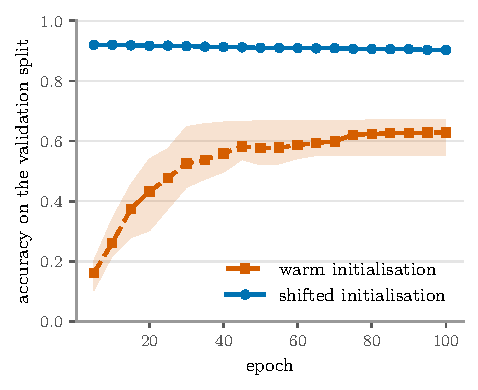
\includegraphics[width=0.44\textwidth]{figures/start_trajectory_accuracy.pdf}\hfill
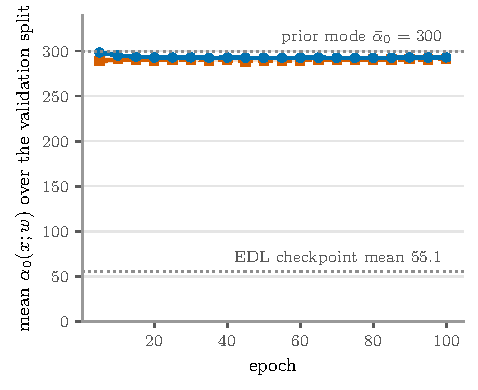
\includegraphics[width=0.44\textwidth]{figures/start_trajectory_alpha0.pdf}
\end{center}
\par\medskip
\begin{itemize}
\item Fashion-MNIST. Prior mode 300. Current weight checkpoints.
\begin{itemize}
\item Lines show means over three seeds. Shading shows the seed range.
\end{itemize}
\end{itemize}
% Preparation. Cat-eBNN on Fashion-MNIST. Means over three seeds. Shading shows the seed range.\par
% Prior mode 300 and prior standard deviation 20\%. Curves use individual weight checkpoints.
% Source detail. Thesis \S5.2.1. These diagnostic curves do not select the reported final BMA.
\end{frame}

% Source. Experiments 5.3.2, fig:count-cold-collapse, tab:e2-count-prior-sensitivity.
% Panels copied unchanged from the thesis figures folder.
\begin{frame}{Backup. Cold initialisation}
\label{frm:backup-collapse}
\begin{center}
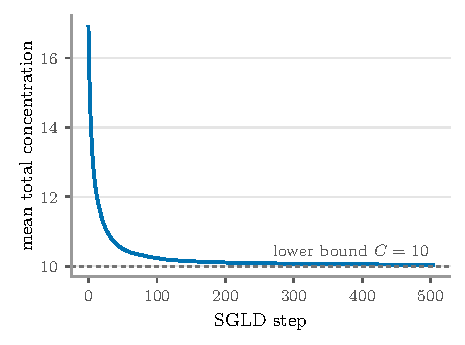
\includegraphics[width=0.44\textwidth]{figures/count_collapse_concentration.pdf}\hfill
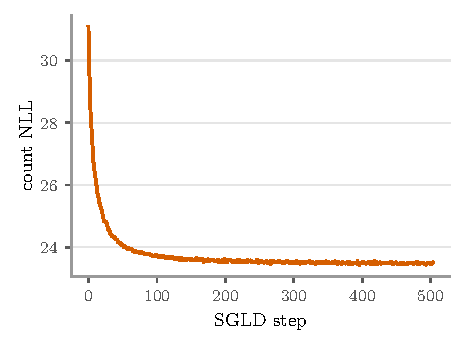
\includegraphics[width=0.44\textwidth]{figures/count_collapse_nll.pdf}
\end{center}
\par\medskip
\begin{itemize}
\item One DM-eBNN run on CIFAR-10H. Cold initialisation without the Gamma prior.
\begin{itemize}
\item Measurements use the current training minibatch before each update.
\end{itemize}
\end{itemize}
% Preparation. One DM-eBNN diagnostic run on CIFAR-10H. Cold initialisation without the Gamma prior.\par
% Measurements precede each update and use the current training minibatch.
% Source detail. Thesis \S5.3.2. The full experiment reports collapse in all three tested cold runs without the Gamma prior.
\end{frame}

% Source. Experiments 5.3.2, fig:count-cold-collapse, tab:e2-count-prior-sensitivity.
% Panels copied unchanged from the thesis figures folder.
\begin{frame}{Backup. Accuracy and gradient norm}
\label{frm:backup-collapse-accuracy}
\begin{center}
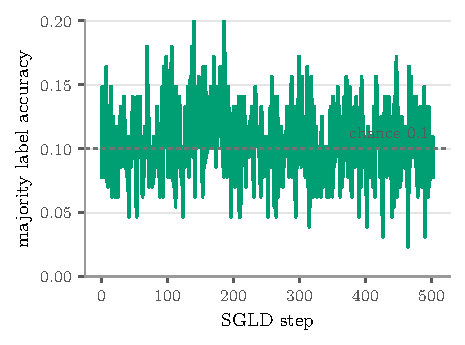
\includegraphics[width=0.44\textwidth]{figures/count_collapse_accuracy.pdf}\hfill
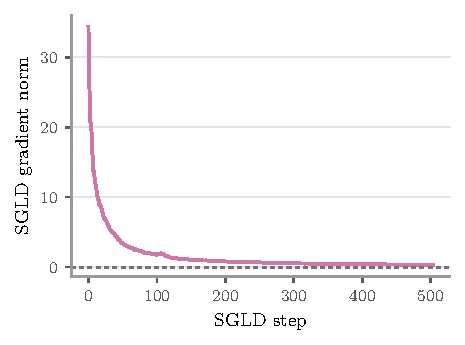
\includegraphics[width=0.44\textwidth]{figures/count_collapse_gradient.pdf}
\end{center}
\par\medskip
\begin{itemize}
\item The same DM-eBNN run without the Gamma prior.
\begin{itemize}
\item The gradient norm falls while majority label accuracy stays near chance.
\end{itemize}
\end{itemize}
% Preparation. The same DM-eBNN diagnostic run on CIFAR-10H. Cold initialisation without the Gamma prior.\par
% The gradient norm falls while majority label accuracy stays near chance.
% Source detail. Thesis \S5.3.2. Current training minibatches, before each update. No BMA.
\end{frame}

